%--------------------------------------------------
%	DOCUMENT IMPORTS
%--------------------------------------------------
\documentclass{beamer}
\usetheme{CambridgeUS}
\usepackage[utf8]{inputenc}
\usepackage[T1]{fontenc}
\usepackage[french]{babel}
\usepackage{graphicx}
\usepackage{xcolor}
\usepackage{tikz}
\usepackage{tkz-graph}
\usepackage{amsmath, amssymb, mathtools, amsthm}
\usepackage{tikz-uml}
%-----------------------------------------------
% DOCUMENT CONFIG
%-----------------------------------------------
\graphicspath{ {figures/} }
\useinnertheme{rectangles}
\setbeamertemplate{blocks}[default]
\usefonttheme[onlymath]{serif}
% Tikz
\tikzstyle{vertex}=[circle, draw, inner sep=2pt, minimum size=8pt, thick]
\newcommand{\vertex}{\node[vertex]}
\usetikzlibrary{arrows,petri,topaths,calc}
% Commands
\newcommand{\yy}[1]{\colorbox{yellow!70}{#1}}
\newcommand{\bb}[1]{\colorbox{blue!30}{#1}}
\newcommand{\rr}[1]{\colorbox{red!30}{#1}}
\newcommand{\gr}[1]{\colorbox{green!30}{#1}}

\title[Pas de jaloux]{Pas de jaloux, un jeu de partage équitable}
\author[Bontems, Mottola, Thirunavukarasu]{Alexandre Bontems \and Gualtiero Mottola \and Hans Thirunavukarasu}
\institute[]{Faculté des Sciences, Sorbonne Université\\Université Pierre et Marie Curie}
\date{5 juin 2018}

\setcounter{tocdepth}{1}
\AtBeginSection[]
{
    \begin{frame}
        \frametitle{Table des matières}
        \tableofcontents[currentsection]
    \end{frame}
}

\begin{document}
\frame{\maketitle}
\section{Introduction}
\begin{frame}
    \frametitle{Présentation du problème LEF}
    \begin{center}
    	Agents : $\{a_1, a_2, a_3, a_4\}$\\
        Objets : $\{o_1, o_2, o_3, o_4\}$
    \end{center}
    \begin{columns}
    	\begin{column}{.49\textwidth}
        	\begin{center}
	    	\begin{tikzpicture}
    	    % Agents
	        \vertex (a1) at (0,0) {$a_1$};
	        \vertex (a2) at (1.5,0) {$a_2$};
	        \vertex (a3) at (3,0) {$a_3$};
	        \vertex (a4) at (4.5,0) {$a_4$};
	        % Prefs
	        \node (a1o1) at (0,2.2) {$o_2$};
	        \node (a1o2) at (0,1.7) {$o_4$};
	        \node (a1o3) at (0,1.2) {$o_1$};
	        \uncover<2->{\node (a1o3) at (0,1.2) {\yy{$o_1$}};}
	        \node (a1o4) at (0,0.7) {$o_3$};
	        \node (a2o1) at (1.5,2.2) {$o_3$};
	        \uncover<2->{\node (a2o1) at (1.5,2.2) {\yy{$o_3$}};}
	        \node (a2o2) at (1.5,1.7) {$o_4$};
	        \node (a2o3) at (1.5,1.2) {$o_2$};
	        \node (a2o4) at (1.5,0.7) {$o_1$};
	        \node (a3o1) at (3.0,2.2) {$o_2$};
	        \uncover<2->{\node (a3o1) at (3.0,2.2) {\yy{$o_2$}};}
	        \node (a3o2) at (3.0,1.7) {$o_1$};
	        \node (a3o3) at (3.0,1.2) {$o_4$};
	        \node (a3o4) at (3.0,0.7) {$o_3$};
	        \node (a4o1) at (4.5,2.2) {$o_3$};
	        \node (a4o2) at (4.5,1.7) {$o_4$};
	        \uncover<2->{\node (a4o2) at (4.5,1.7) {\yy{$o_4$}};}
	        \node (a4o3) at (4.5,1.2) {$o_2$};
	        \node (a4o4) at (4.5,0.7) {$o_1$};
	        \path
	        (a1) edge[thick] (a2)
            (a2) edge[thick] (a3)
            (a3) edge[thick] (a4)       
	        ;
	   		\end{tikzpicture}
			\end{center}
        \end{column}~
        \begin{column}{.49\textwidth}
        	\begin{itemize}
            	\item Agents liés dans un réseau
            	\item Un objet par agent
                \item Préférences distinctes
            	\item Problème de satisfaction NP-complet
            \end{itemize}
        \end{column}
    \end{columns}
	
\end{frame}

\begin{frame}
\frametitle{Objectifs}
\begin{center}
Développement d'un jeu puzzle basé sur le problème et offrant une progression de difficulté.\\[0.5cm]
\end{center}
\begin{columns}
\centering
\begin{column}{.49\textwidth}
\uncover<2->{
\begin{block}{Exigences}
\begin{itemize}
    \item Produire un jeu,
    \item Obtenir des niveaux possédant au moins une solution,
    \item Connaître la difficulté des niveaux,
\end{itemize}
\end{block}
}
\end{column}
\begin{column}{0.49\textwidth}
\uncover<2->{
\begin{block}{Solutions}
\begin{itemize}
    \item Application Android
    \item Outils d'analyse de difficulté
    \item Taille des instances bornée
\end{itemize}
\end{block}
}
\end{column}
\end{columns}
\end{frame}

\section{Application}

\subsection{Conception de l'interface}
\begin{frame}
\frametitle{Analyse des besoins utilisateurs}
\begin{itemize}
	\item Qui sont nos utilisateurs?
    \begin{itemize}
    	\item Public visé large
        \item Ne pas introduire de biais
    \end{itemize}
    \item Récoltes de données sur nos utilisateurs
    \begin{itemize}
    	\item Interviews
        \item Analyse d'applications de jeux connues
    \end{itemize}
    \item Emergence des tâches systèmes de notre application
\end{itemize}
\end{frame}

\begin{frame}
\frametitle{Objectifs de notre interface}
\begin{itemize}
	\item Une interface claire et épurée
    \item Le nombre d'informations affichées à l'écran
    \item Rapidité et fluidité de notre interface
\end{itemize}
\end{frame}

\begin{frame}
\frametitle{Critères d'évaluation}
\begin{itemize}
	\item Facilité d'usage "Easy to use"
    \item Facilité d'apprentissage "Easy to learn"
    \item Satisfaction personnelle
\end{itemize}
\end{frame}

\begin{frame}
\frametitle{Evolution des designs de notre interface}
\begin{center}
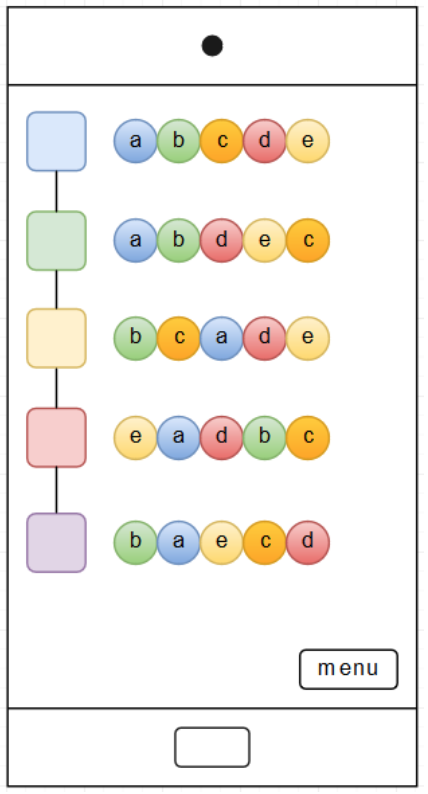
\includegraphics[width=0.29\textwidth]{maquette}~
\raisebox{.65\height}{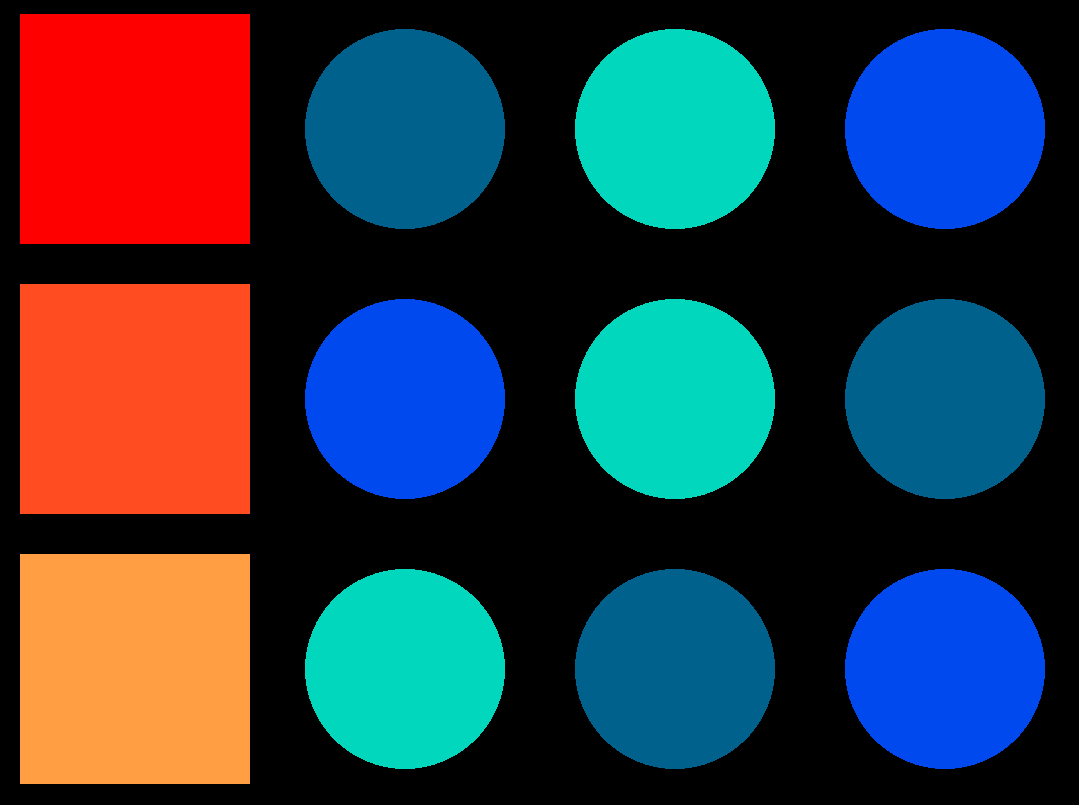
\includegraphics[width=0.29\textwidth]{prototype1}}~
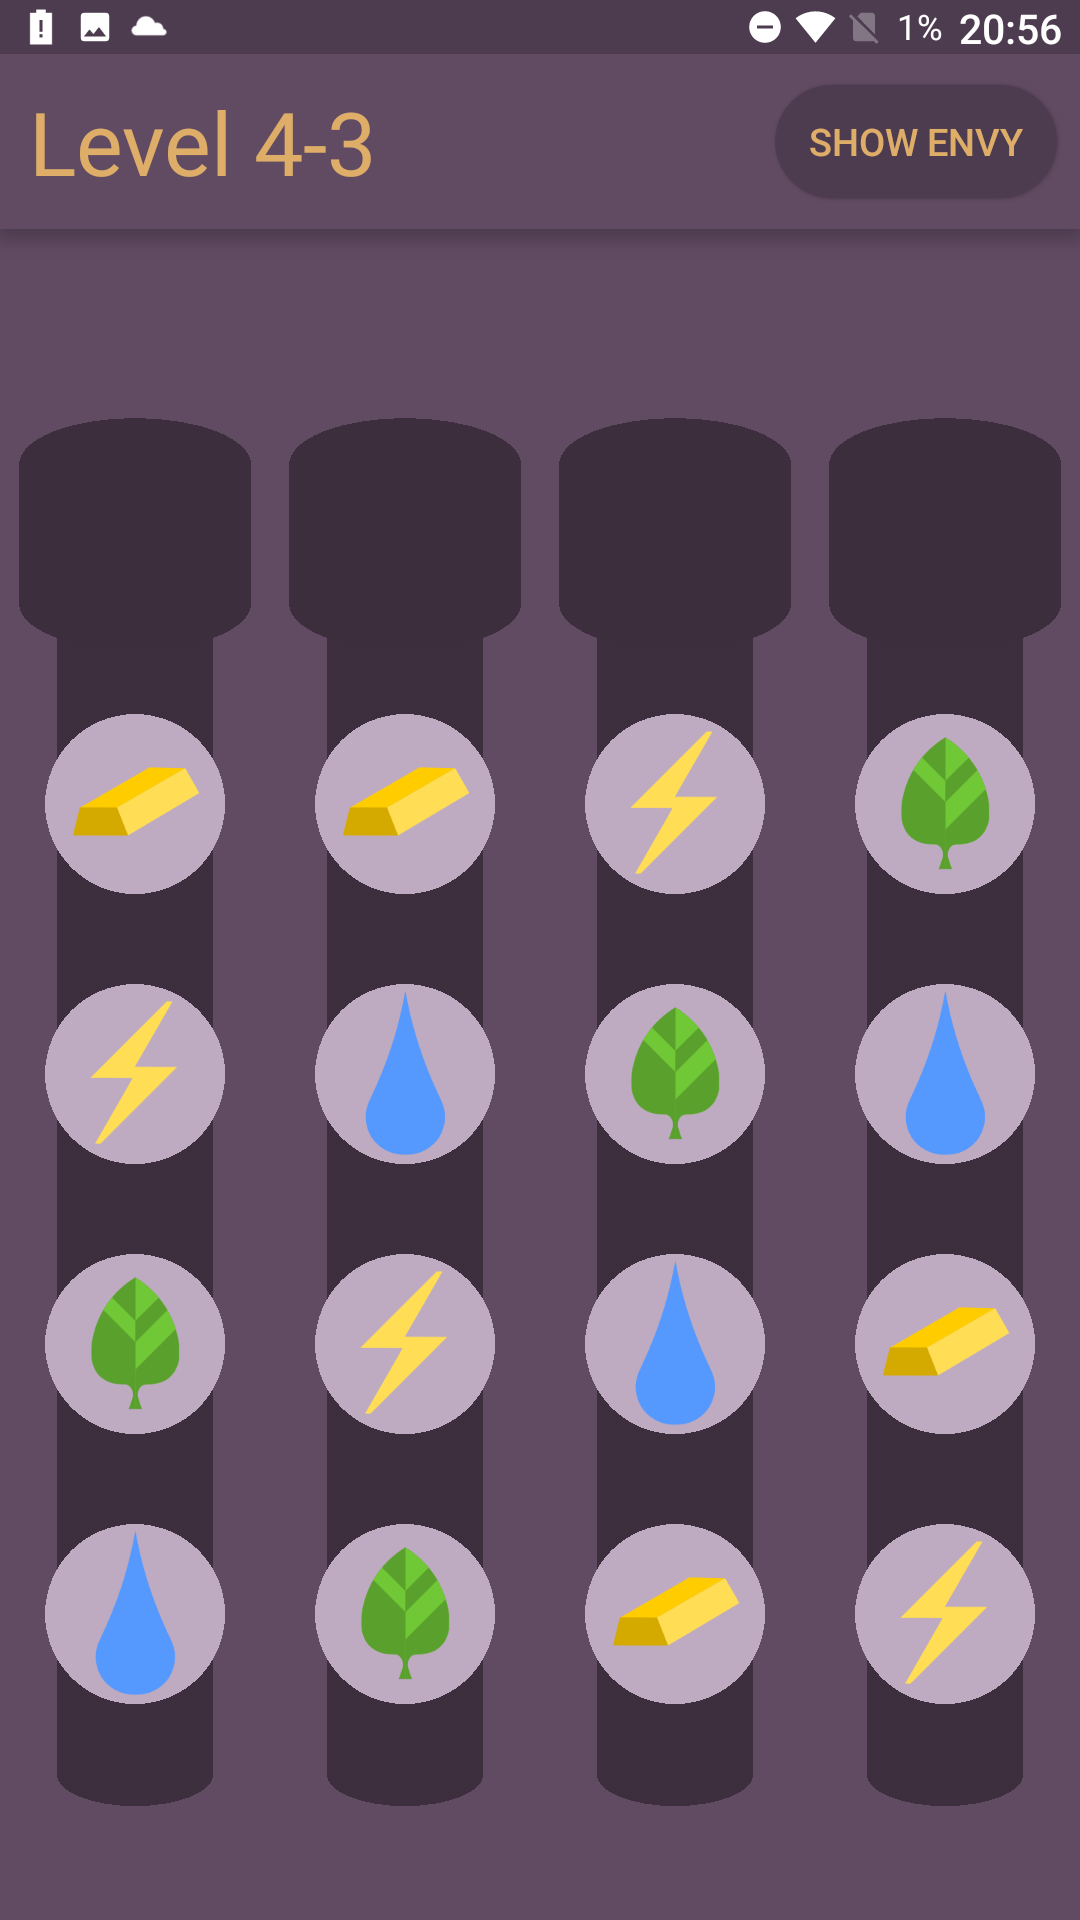
\includegraphics[width=0.29\textwidth]{g1}
\end{center}
\end{frame}

\begin{frame}
\frametitle{Fonctionnement de l'interface finale}
\begin{columns}
\begin{column}{0.45\textwidth}
   \begin{itemize}
	\item Nom du niveau et bouton d'affichage d'envie
    \item Affichage des selections doubles  
    \item Surbrillance des acteur envieux  
\end{itemize}
\end{column}~
\begin{column}{0.49\textwidth}
    \begin{center}
     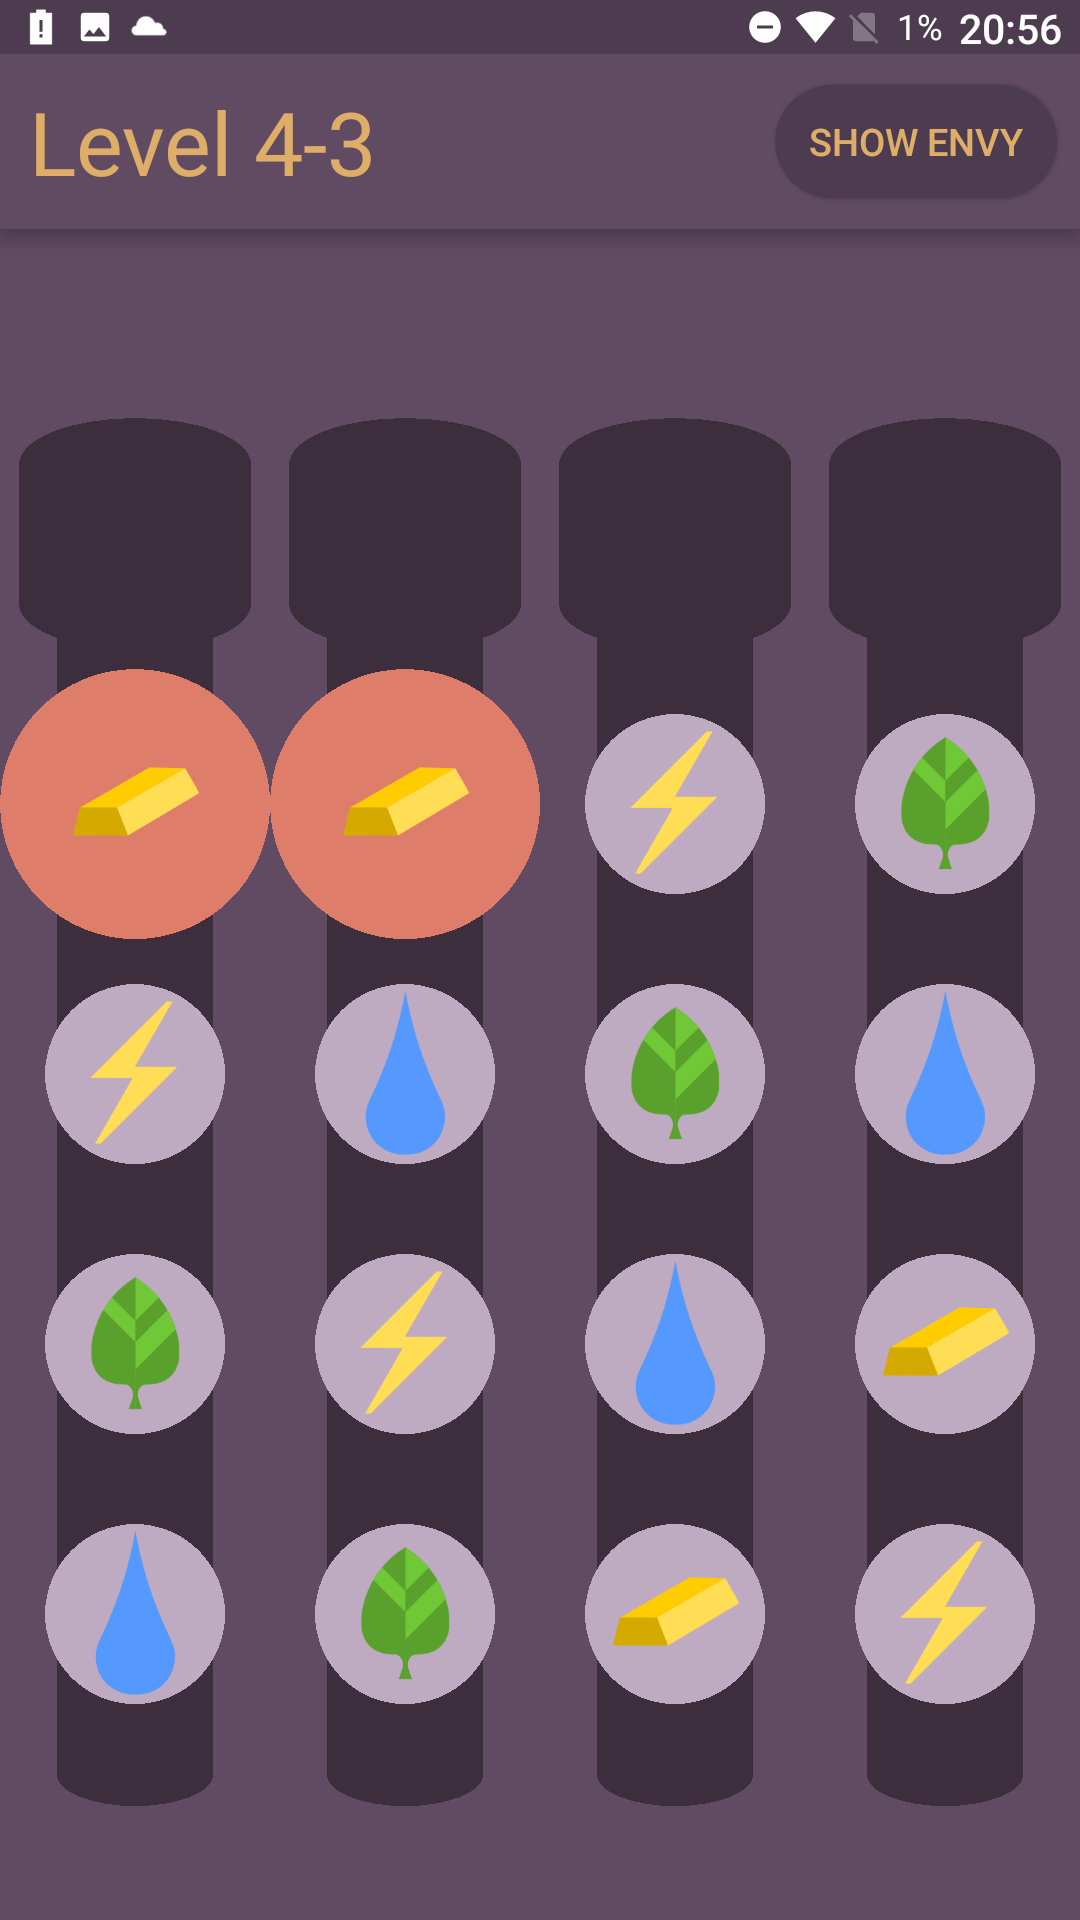
\includegraphics[width=0.49\textwidth]{g2}
     ~
     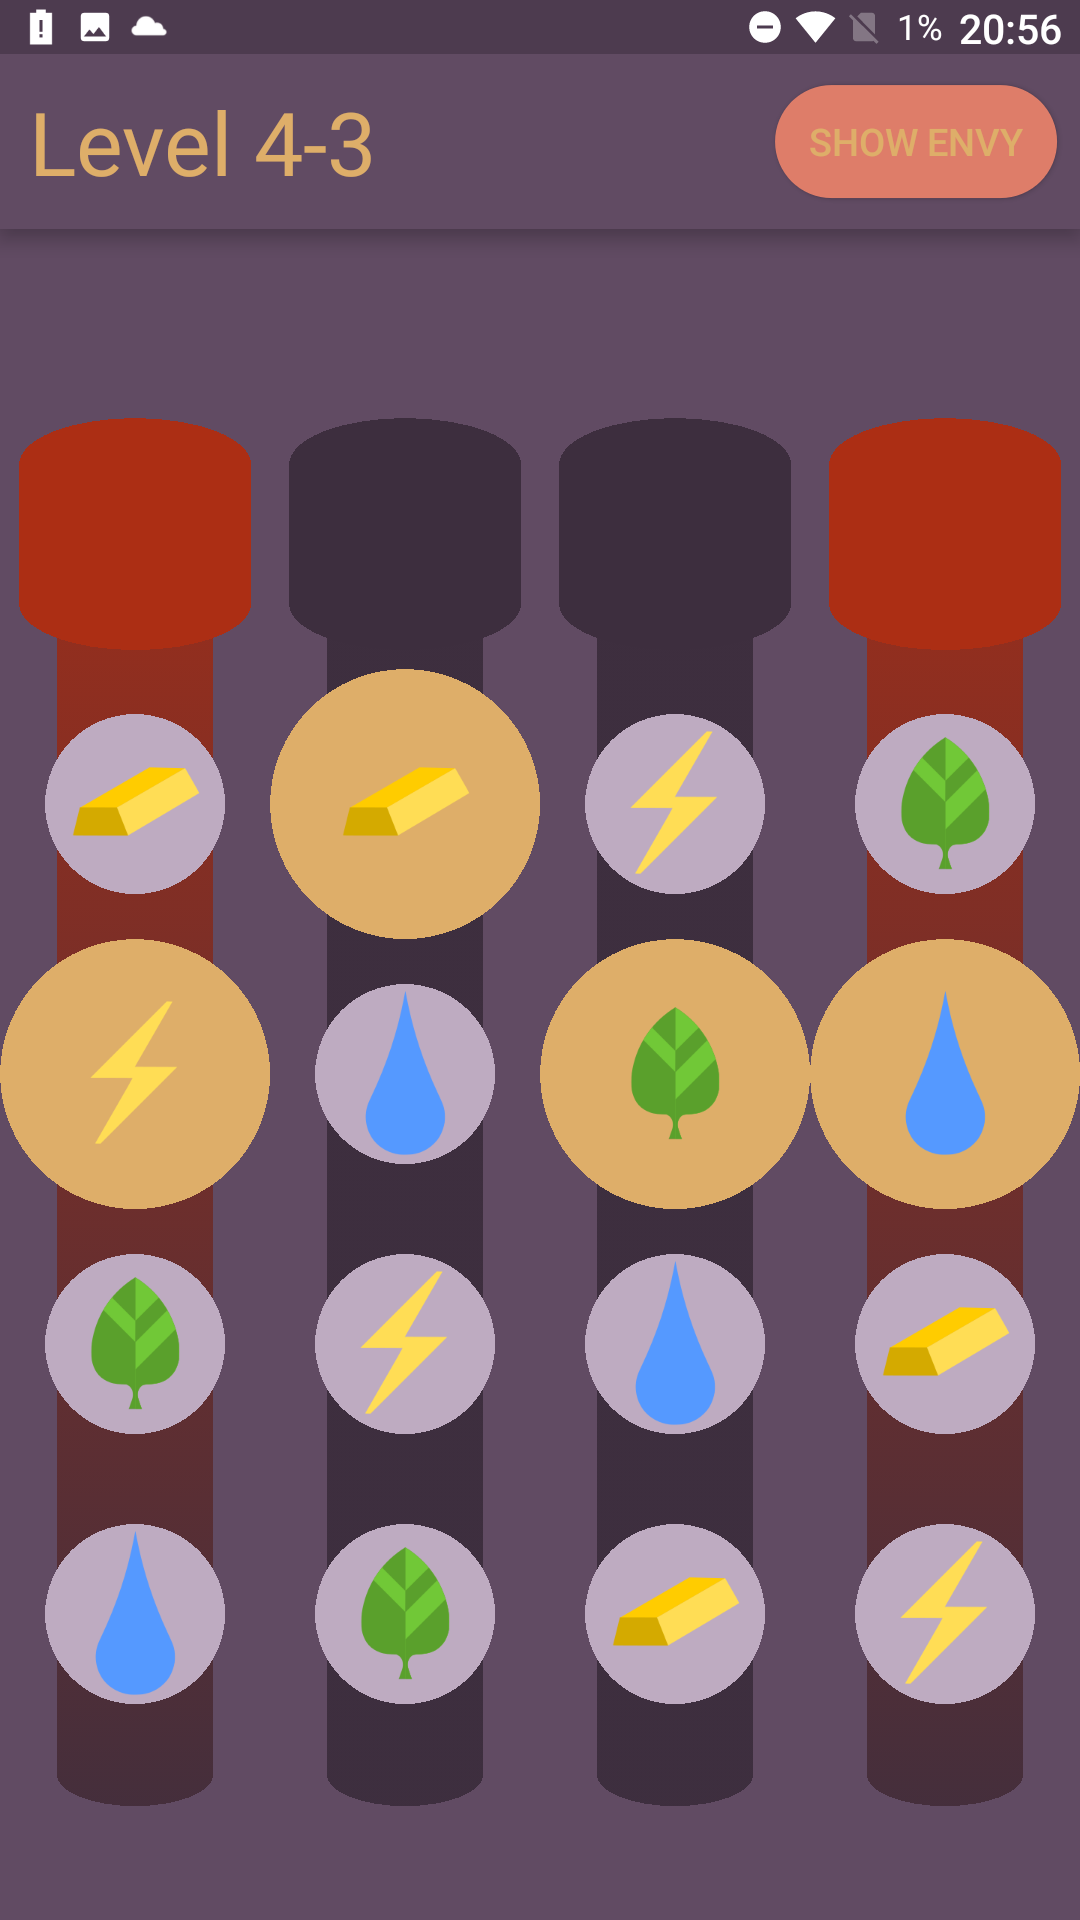
\includegraphics[width=0.49\textwidth]{g3}   
     \end{center}
\end{column}
\end{columns}
\end{frame}

\begin{frame}
\frametitle{Notation des niveaux}
\begin{columns}
\begin{column}{0.49\textwidth}
   \begin{itemize}
	\item Détection de la victoire automatique
    \item Popup d'affichage 
    \item Système a base d'etoiles
    \item Notation du niveau obligatoire
\end{itemize}
\end{column}~
\begin{column}{0.49\textwidth}
    \begin{center}
     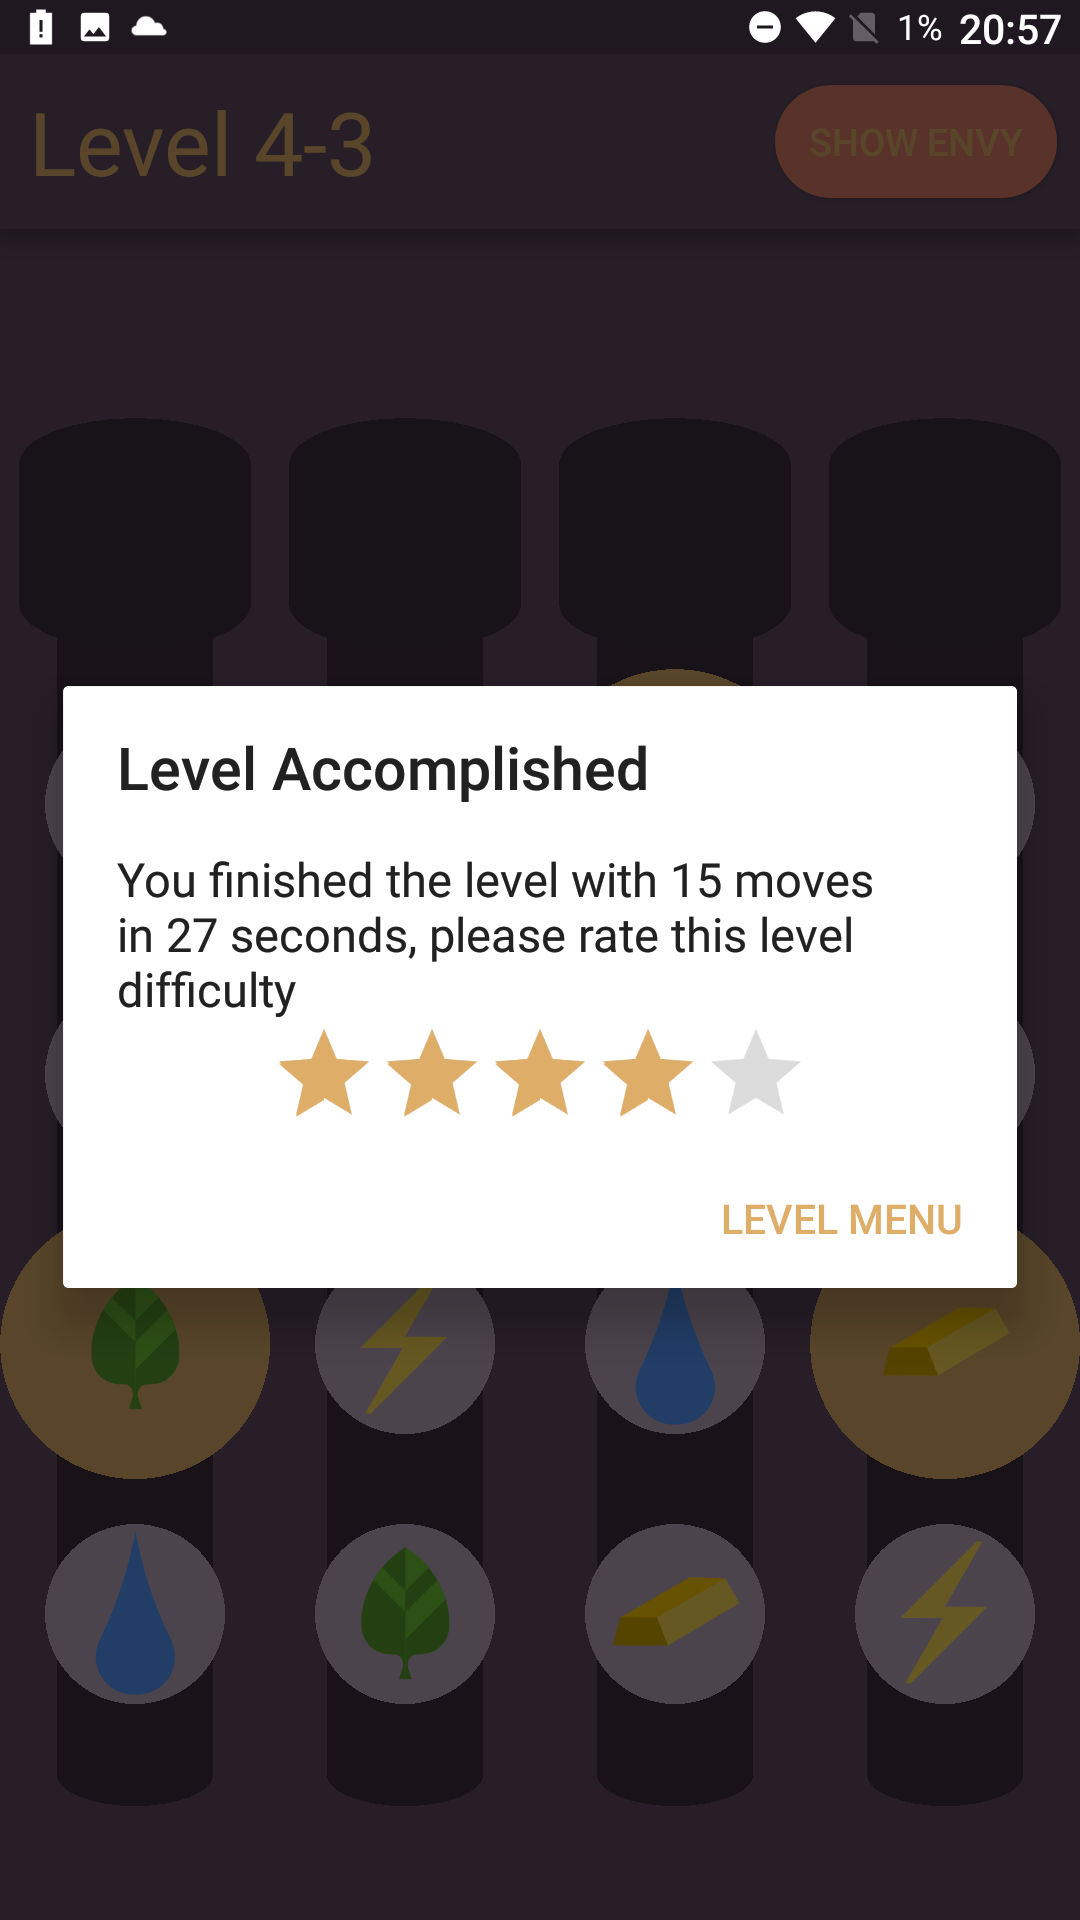
\includegraphics[width=0.55\textwidth]{g4}
     \end{center}
\end{column}
\end{columns}
\end{frame}

\begin{frame}
\frametitle{Tutoriel}
\begin{columns}
\begin{column}{0.49\textwidth}
   \begin{itemize}
	\item Description de l'interface
    \item Explication du concept de jalousie 
    \item Conditions de victoire 
\end{itemize}
\end{column}~
\begin{column}{0.49\textwidth}
    \begin{center}
     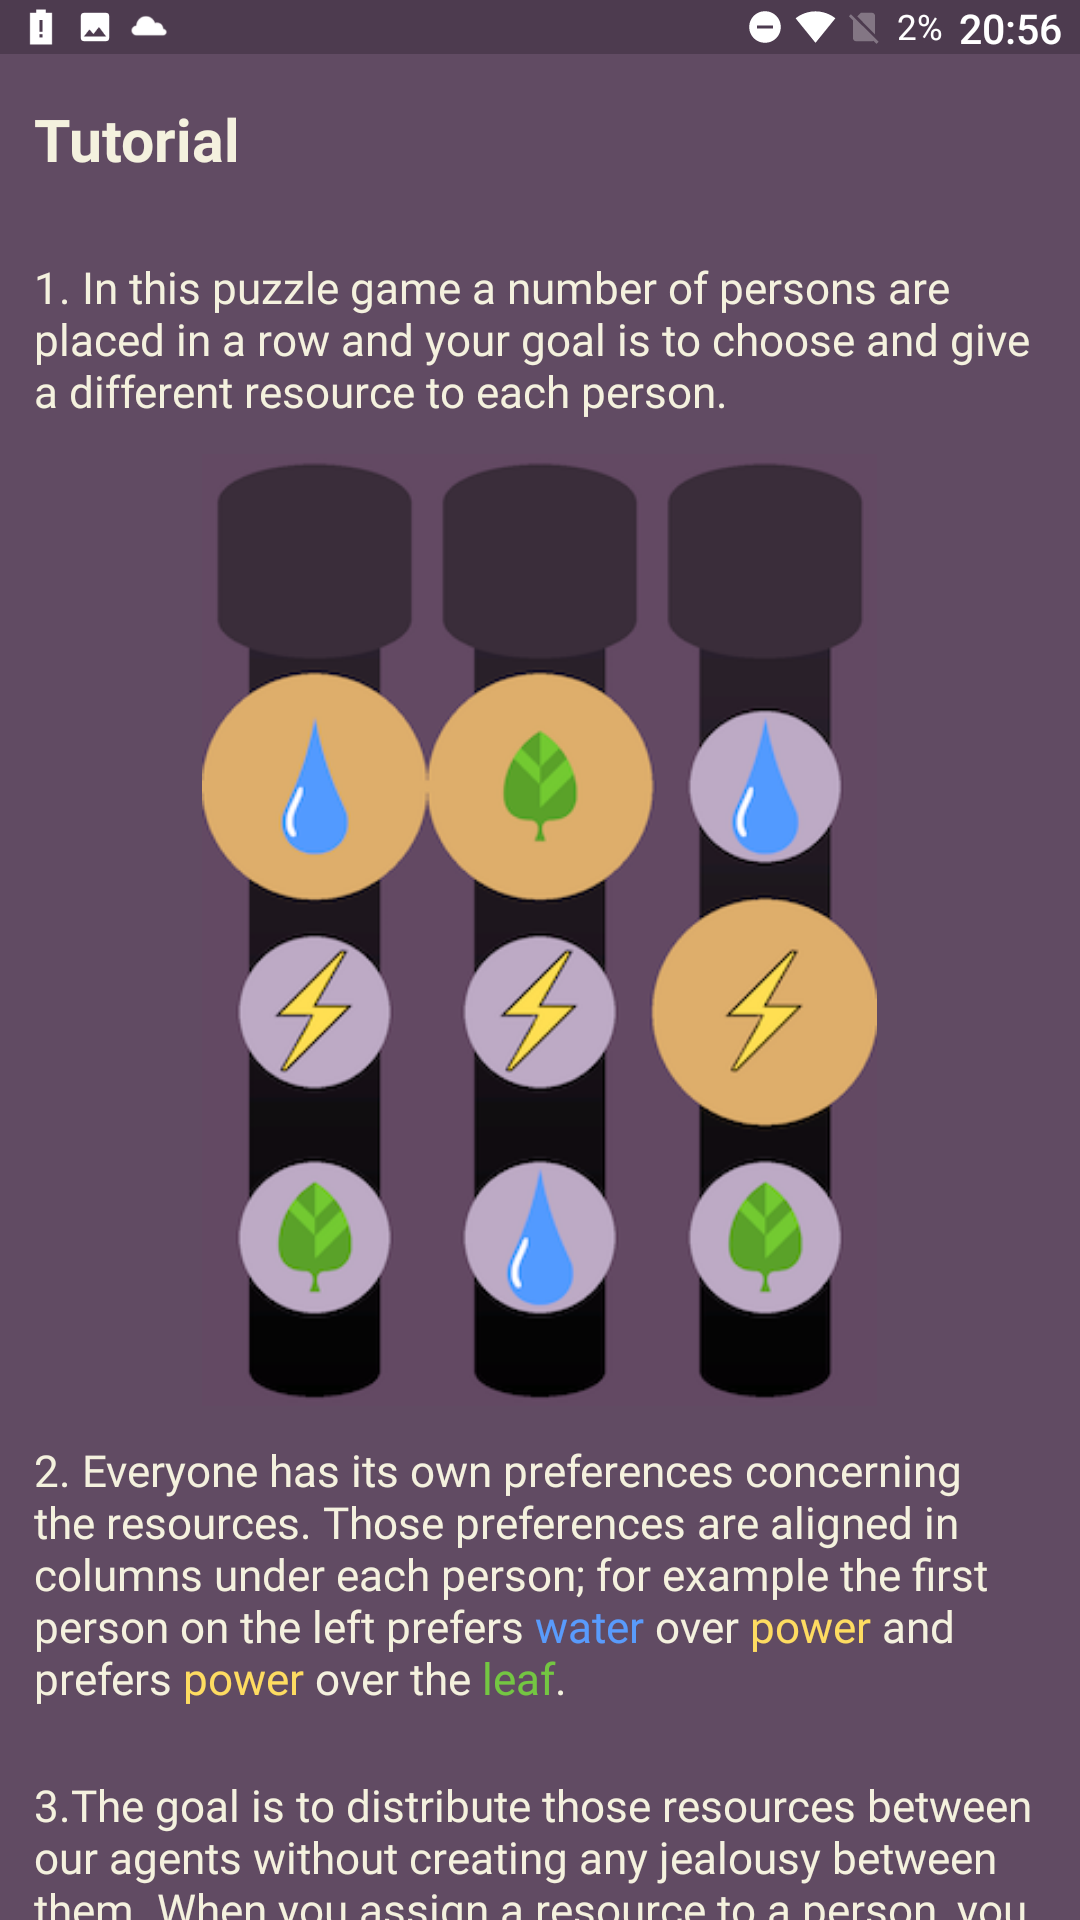
\includegraphics[width=0.55\textwidth]{tuto}
     \end{center}
\end{column}
\end{columns}
\end{frame}

\begin{frame}
\frametitle{Structure de l'interface}
\centering
\resizebox{12cm}{!}{
\begin{tikzpicture}
    \umlsimpleclass{MainMenuActivity}
    \umlsimpleclass[x=6]{LevelMenuActivity}
    \umlsimpleclass[x=12]{GameActivity}
    \umlsimpleclass[y=2]{TutorialActivity}
    \umlsimpleclass[y=-2]{UserProfileActivity}
    \umlsimpleclass[y=-2, x=6]{AboutActivity}
    
    \umlassoc{MainMenuActivity}{TutorialActivity}
    \umlassoc{MainMenuActivity}{UserProfileActivity}
    \umlassoc{MainMenuActivity}{LevelMenuActivity}
    \umlassoc{MainMenuActivity}{AboutActivity}
    \umlassoc{LevelMenuActivity}{GameActivity}
\end{tikzpicture}
}
\end{frame}


\begin{frame}
\frametitle{Autres Activités}
\begin{columns}
\begin{column}{0.49\textwidth}
   \begin{itemize}
	\item Entrée des informations testeurs 
    \item Première Activité lors de l'ouverture l'application  
    \item Acessible depuis le menu principal
    \item Affichage des niveaux complétés
    \item Affichage des niveaux en cours
\end{itemize}
\end{column}~
\begin{column}{0.49\textwidth}
    \begin{center}
     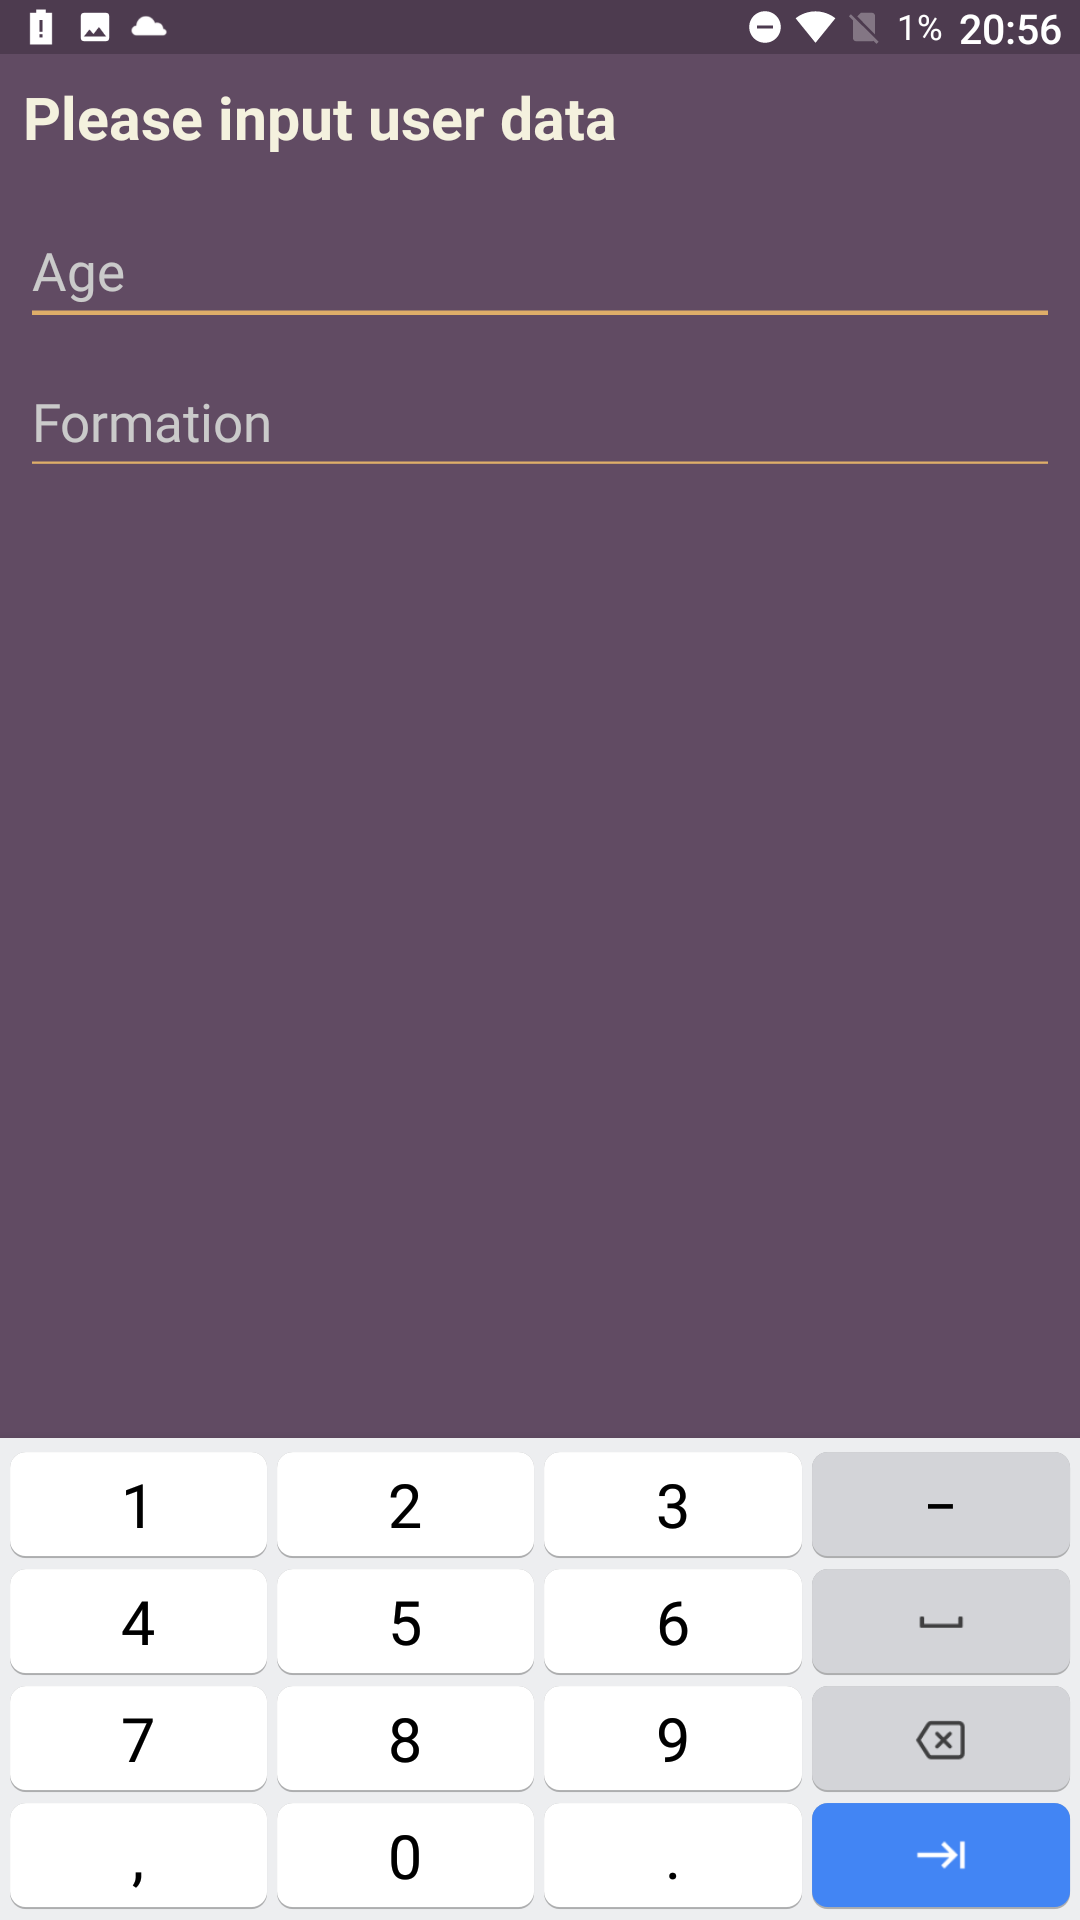
\includegraphics[width=0.49\textwidth]{infor}
     ~
     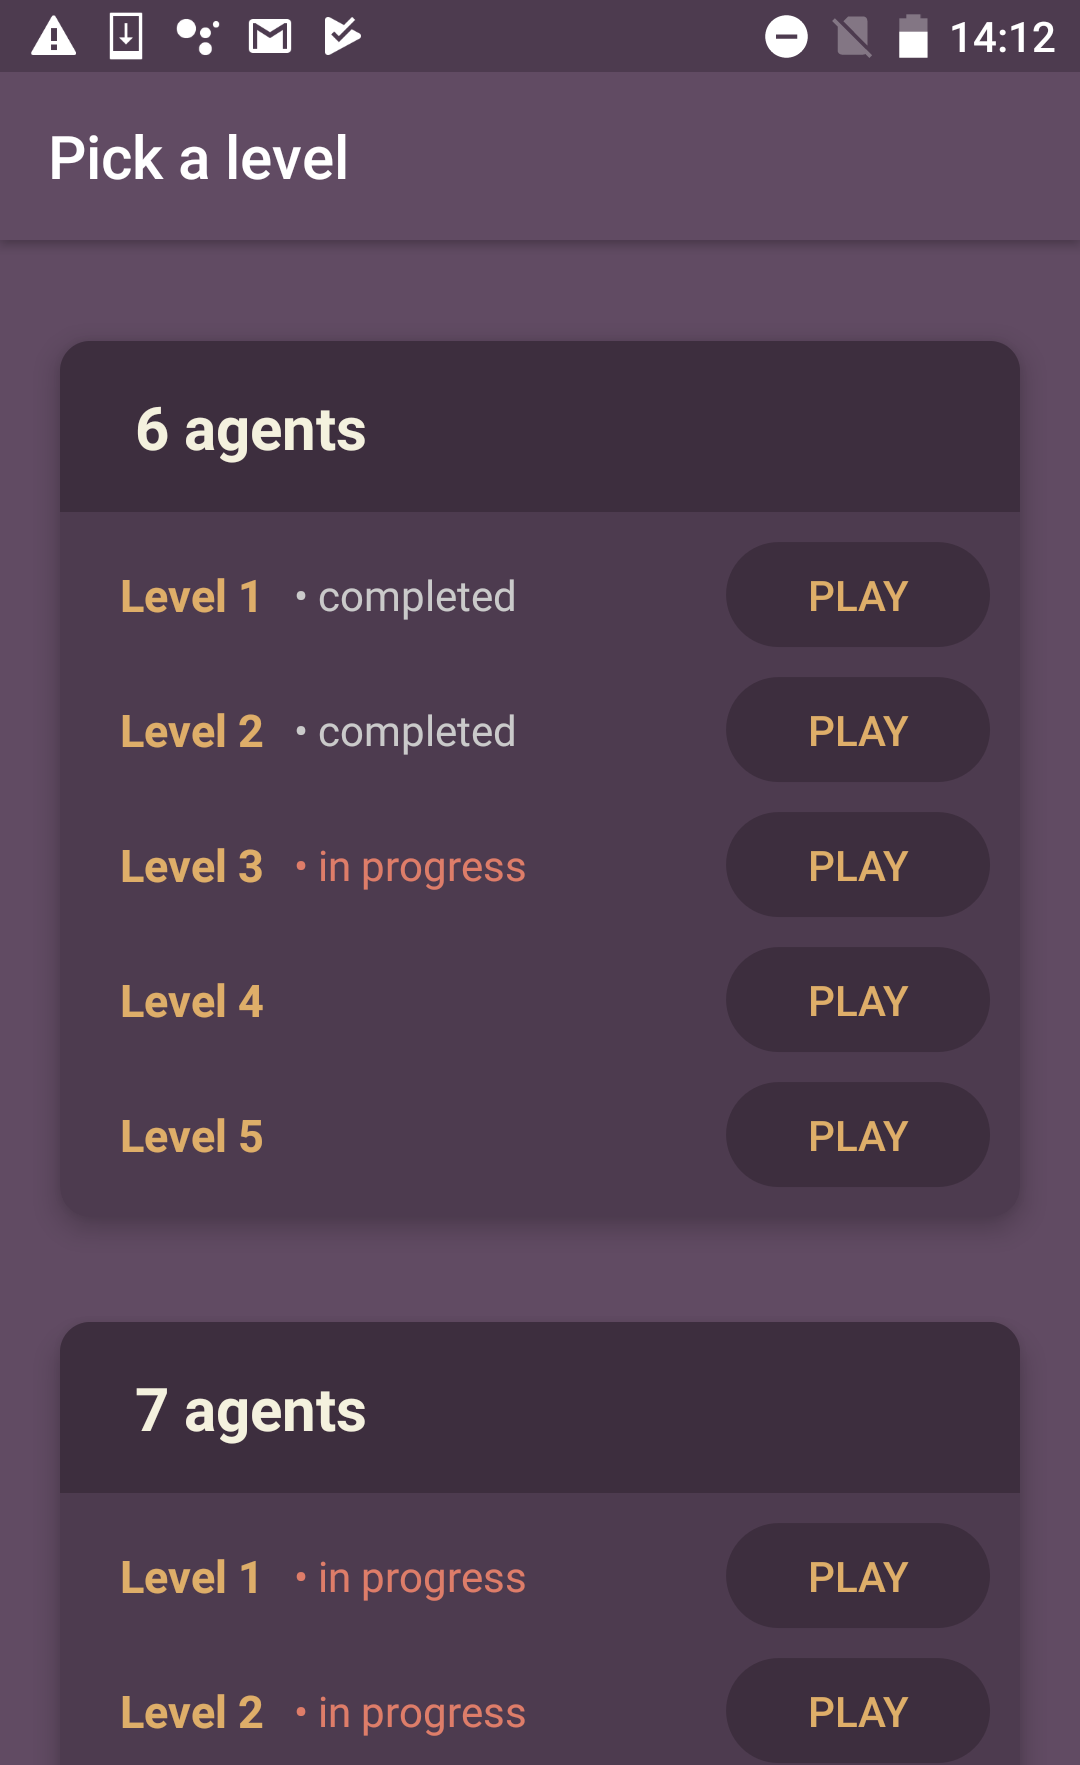
\includegraphics[width=0.49\textwidth]{levelmenu}   
     \end{center}
\end{column}
\end{columns}
\end{frame}


\subsection{Architecture}
\begin{frame}
\frametitle{Structure du Back-End}
\centering
\resizebox{6cm}{!}{
\begin{tikzpicture}
    \begin{umlpackage}{Models}
        \umlsimpleclass{Grid}
        \umlsimpleclass[y=-2]{Model}
        \umlassoc[mult2=1, mult1=1]{Model}{Grid}
        \umlsimpleclass[y=-4]{Level}
        \umlassoc[mult2=1, mult1=1]{Model}{Level}
        \umlsimpleinterface[x=3,y=-2]{IPiece}
        \umlassoc[mult1=1,mult2=*]{Model}{IPiece}
        \umlsimpleclass[x=2.5, y=-4]{Actor}
        \umlsimpleclass[x=5, y=-4]{Preference}
        \umlimpl{Actor}{IPiece}
        \umlimpl{Preference}{IPiece}
        \umlsimpleclass[x=4, y=-6.5]{Position}
        \umlassoc[mult1=1, mult2=1]{Actor}{Position}
        \umlassoc[mult1=1, mult2=1]{Preference}{Position}
    \end{umlpackage}
\end{tikzpicture}
}
\end{frame}


\begin{frame}
\frametitle{Intégration GoogleSheets}
\centering
\resizebox{12cm}{!}{
\begin{tikzpicture}
    \begin{umlpackage}[fill=red!20]{GoogleSheets}
        \umlsimpleclass{GoogleSheetsWriteUtil}
        \umlsimpleclass[y=-1.5]{SheetsServiceUtil}
        \umluniassoc{GoogleSheetsWriteUtil}{SheetsServiceUtil}
        \umlsimpleclass[x=6, type=abstract]{AsyncTask}
        \umluniassoc{GoogleSheetsWriteUtil}{AsyncTask}
        \umlsimpleclass[y=-2, x=4]{WriteUserInfo}
        \umlimpl{WriteUserInfo}{AsyncTask}
        \umlsimpleclass[y=-2, x=8]{WriteUserEvaluation}
        \umlimpl{WriteUserEvaluation}{AsyncTask}
        \umlsimpleclass[x=10]{ModifyUserProfile}
        \umlimpl{ModifyUserProfile}{AsyncTask}
    \end{umlpackage}
\end{tikzpicture}
}
\end{frame}



\subsection{Récupération des données}
\begin{frame}
\frametitle{Intégration GoogleSheets}
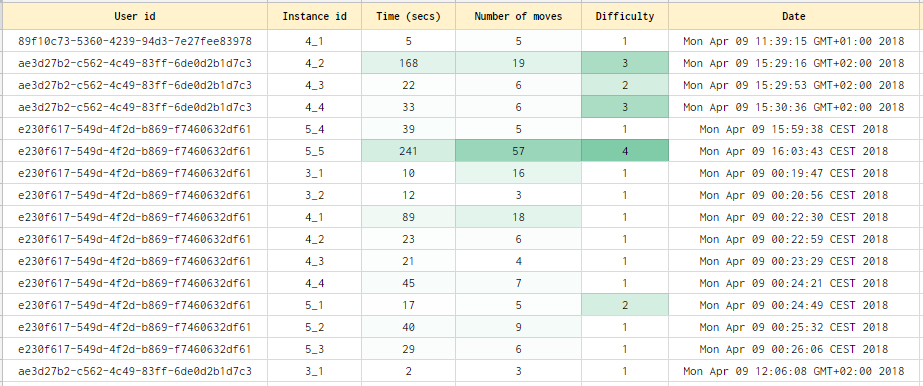
\includegraphics[width=1\textwidth]{Sheets}
\end{frame}

\section{Analyse}
\begin{frame}
\frametitle{Génération d'instances solvables}
\centering
\begin{tikzpicture}
    	    % Agents
	        \vertex (a1) at (0,0) {$a_1$};
	        \vertex (a2) at (1.5,0) {$a_2$};
	        \vertex (a3) at (3,0) {$a_3$};
	        \vertex (a4) at (4.5,0) {$a_4$};
	        % Prefs
	        \node (a1o1) at (0,2.2) {$o_3$};
	        \node (a1o2) at (0,1.7) {$o_4$};
	        \node (a1o3) at (0,1.2) {\fbox{$o_1$}};
	        \node (a1o4) at (0,0.7) {\bb{$o_2$}};
	        \node (a2o1) at (1.5,2.2) {\fbox{$o_2$}};
	        %\uncover<2->{\node (a2o1) at (1.5,2.2) {\yy{$o_3$}};}
	        \node (a2o2) at (1.5,1.7) {$o_4$};
	        \node (a2o3) at (1.5,1.2) {\bb{$o_3$}};
	        \node (a2o4) at (1.5,0.7) {\bb{$o_1$}};
	        \node (a3o1) at (3.0,2.2) {\fbox{$o_3$}};
	        %\uncover<2->{\node (a3o1) at (3.0,2.2) {\yy{$o_2$}};}
	        \node (a3o2) at (3.0,1.7) {$o_1$};
	        \node (a3o3) at (3.0,1.2) {\bb{$o_4$}};
	        \node (a3o4) at (3.0,0.7) {\bb{$o_2$}};
	        \node (a4o1) at (4.5,2.2) {$o_2$};
	        \node (a4o2) at (4.5,1.7) {\fbox{$o_4$}};
	        %\uncover<2->{\node (a4o2) at (4.5,1.7) {\yy{$o_4$}};}
	        \node (a4o3) at (4.5,1.2) {\bb{$o_3$}};
	        \node (a4o4) at (4.5,0.7) {$o_1$};
	        \path
	        (a1) edge[thick] (a2)
            (a2) edge[thick] (a3)
            (a3) edge[thick] (a4)       
	        ;
\end{tikzpicture}
\vspace{1cm}
\begin{columns}
\centering
\begin{column}{.6\textwidth}
\begin{itemize}
	\item Choix d'une allocation
    \item Placement des objets voisins
    \item Placement aléatoire des objets restants
\end{itemize}
\end{column}
\end{columns}
\end{frame}

\begin{frame}
\frametitle{Résolution par backtrack}
\centering
		\begin{tabular}{c|c c c c c c c}
		    \textbf{Index} \\
			\hline
			0&    2	& \yy{3}	& \yy{2}	& \yy{5} & \yy{7}	& \yy{4}	& \yy{6}	\\ 
    		1&  \yy{1} &  4    &  6	&  6	&  3    & \bb{5}&  1	\\ 
			2&    3	&  2	& \bb{1}&  7	& \bb{2}&  6    & \bb{3}\\ 
			3& \bb{6}	&  5	&  3	&  3    &  1	&  7	&  7	\\ 
			4&    5	& \bb{7}&  4	& \bb{4}&  6	&  1	&  5	\\ 
			5&    3	&  1	&  7	&  2	&  4	&  2	&  2	\\ 
			6&    7	&  6	&  5	&  1	&  5	&  3	&  4    \\ 
			\hline
\end{tabular}\\[0.8cm]
Regret minimum, regret moyen, regret extrêmité, nombre d'affectation, solutions Pareto-optimales.
\end{frame}

\begin{frame}
\frametitle{Résolution ASP}
\centering
Récupération de l'ensemble des solutions d'une instance\\[0.2cm]
\begin{itemize}
	\item Génération: un objet par agent\\[.1cm]
    \texttt{1\{ aff(A, O) : object(O) \}1 :- agent(A).}
    
    \uncover<2->{\item Un agent par objet\\[.1cm]
    \texttt{:- aff(A1, O), aff(A2, O), A1 != A2.}}
    
    \uncover<3->{\item Pas de jalousie\\[.1cm]
    \texttt{:- aff(A1, O1), aff(A2, O2),\\
	position(A1, O1, P1), \\
	position(A1, O2, P2), \\
	P2 < P1, voisins(A1,A2).}}
\end{itemize}
\uncover<4->{Nombre total de solutions, nombre de variables frozen.}
\end{frame}

\begin{frame}
\frametitle{Analyse de fitness landscape}
\centering
\includegraphics<1>[width=0.8\textwidth]{basin-5-2}
\includegraphics<2>[width=0.8\textwidth]{basin_7-6}
\end{frame}

\begin{frame}
\frametitle{Apprentissage}
\end{frame}

\section{Conclusion}

\begin{frame}
\frametitle{Travail futur}
 \begin{itemize}
 	\item Plus de mesures 
    \item Ameliorer les modèles d'apprentissage  
   	\item Déploiement de l'application sur PlayStore
   	\item Chargement des niveaux à distance
    \item Changer la disposition des agents
  	\item Obstruer la visibilité de certains agents
  	\item Implementation iOS 
\end{itemize}
\end{frame}


\begin{frame}
\frametitle{Merci}
 \begin{itemize}
   \item Mottola Gualtiero (\url{gualt1995@gmail.com})
   \item Bontems Alexandre (\url{alexandre.bontems@gmail.com})
   \item Thirunavukarasu Hans (\url{hans.thiru@gmail.com})
\end{itemize}
\end{frame}
\end{document}